\documentclass[]{article}
\renewcommand{\baselinestretch}{1.25}

\usepackage[margin=1in]{geometry}
\usepackage{physics}
\usepackage{amsmath, amsfonts, amssymb, amsthm}
\usepackage{amssymb}
\usepackage{graphicx}
\usepackage{hyperref}
\usepackage{empheq}
\usepackage{pdfpages}
\usepackage{xcolor}
\usepackage{ulem}

% MATLAB Formatting Code
\usepackage[numbered,framed]{matlab-prettifier}
\lstset{style=Matlab-editor,columns=fullflexible}
\renewcommand{\lstlistingname}{Script}
\newcommand{\scriptname}{\lstlistingname}

% TikZ Things
\usepackage{tikz}
\usetikzlibrary{positioning,shapes}


% Formatting Preferences
\numberwithin{equation}{section}
\usepackage{parskip}
\renewcommand{\figurename}{Fig.}
\allowdisplaybreaks

% Section Heading Settings
\usepackage{enumitem}
\renewcommand{\theenumi}{\alph{enumi}}
\renewcommand*{\thesection}{Problem \arabic{section}}
\renewcommand*{\thesubsection}{\alph{subsection})}
\renewcommand*{\thesubsubsection}{\quad \quad \roman{subsubsection})}

% Math Proof things
\newcommand{\Rel}{\mathcal{R}}
\newcommand{\R}{\mathbb{R}}
\newcommand{\C}{\mathbb{C}}
\newcommand{\N}{\mathbb{N}}
\newcommand{\Z}{\mathbb{Z}}
\newcommand{\Q}{\mathbb{Q}}

\newcommand{\st}{\ : \ }

% Theorem Definition
\newtheorem{definition}{Definition}
\newtheorem{assumption}{Assumption}
\newtheorem{theorem}{Theorem}
\newtheorem{lemma}{Lemma}
\newtheorem{proposition}{Proposition}
\newtheorem{example}{Example}


% Multiagent Robotic Systems Commands
\newcommand{\diam}{\textnormal{diam}}
\newcommand{\radius}{\textnormal{radius}}




%opening
\title{MECH 6V29: Multiagent Robotic Systems- HW 3}
\author{Jonas Wagner}
\date{2022, March 22\textsuperscript{nd}}

\begin{document}	

\maketitle

\tableofcontents

%----------------------------------------------------------------------------

% Problem 1 -------------------------------------------------
\newpage
\section{}
% \textbf{Problem:} 
State a summary of \emph{\textbf{Notes 11, 12 and 13}}, preferably by creating a concept map diagram (flow diagram). 
The whole purpose is to make sure that we are clear about the bigger picture, 
and reiterate why are we doing and discussing the specific topics in the class. 
Do not merely write the topics, instead create connections between topics to clarify the flow of information.

\textbf{Note:} 
Since we have only covered Notes 11 and 12, this chart only includes those topics.

\subsection{Big Picture Chart}
\begin{figure}[h]
	\centering
    \resizebox*{\textwidth}{!}{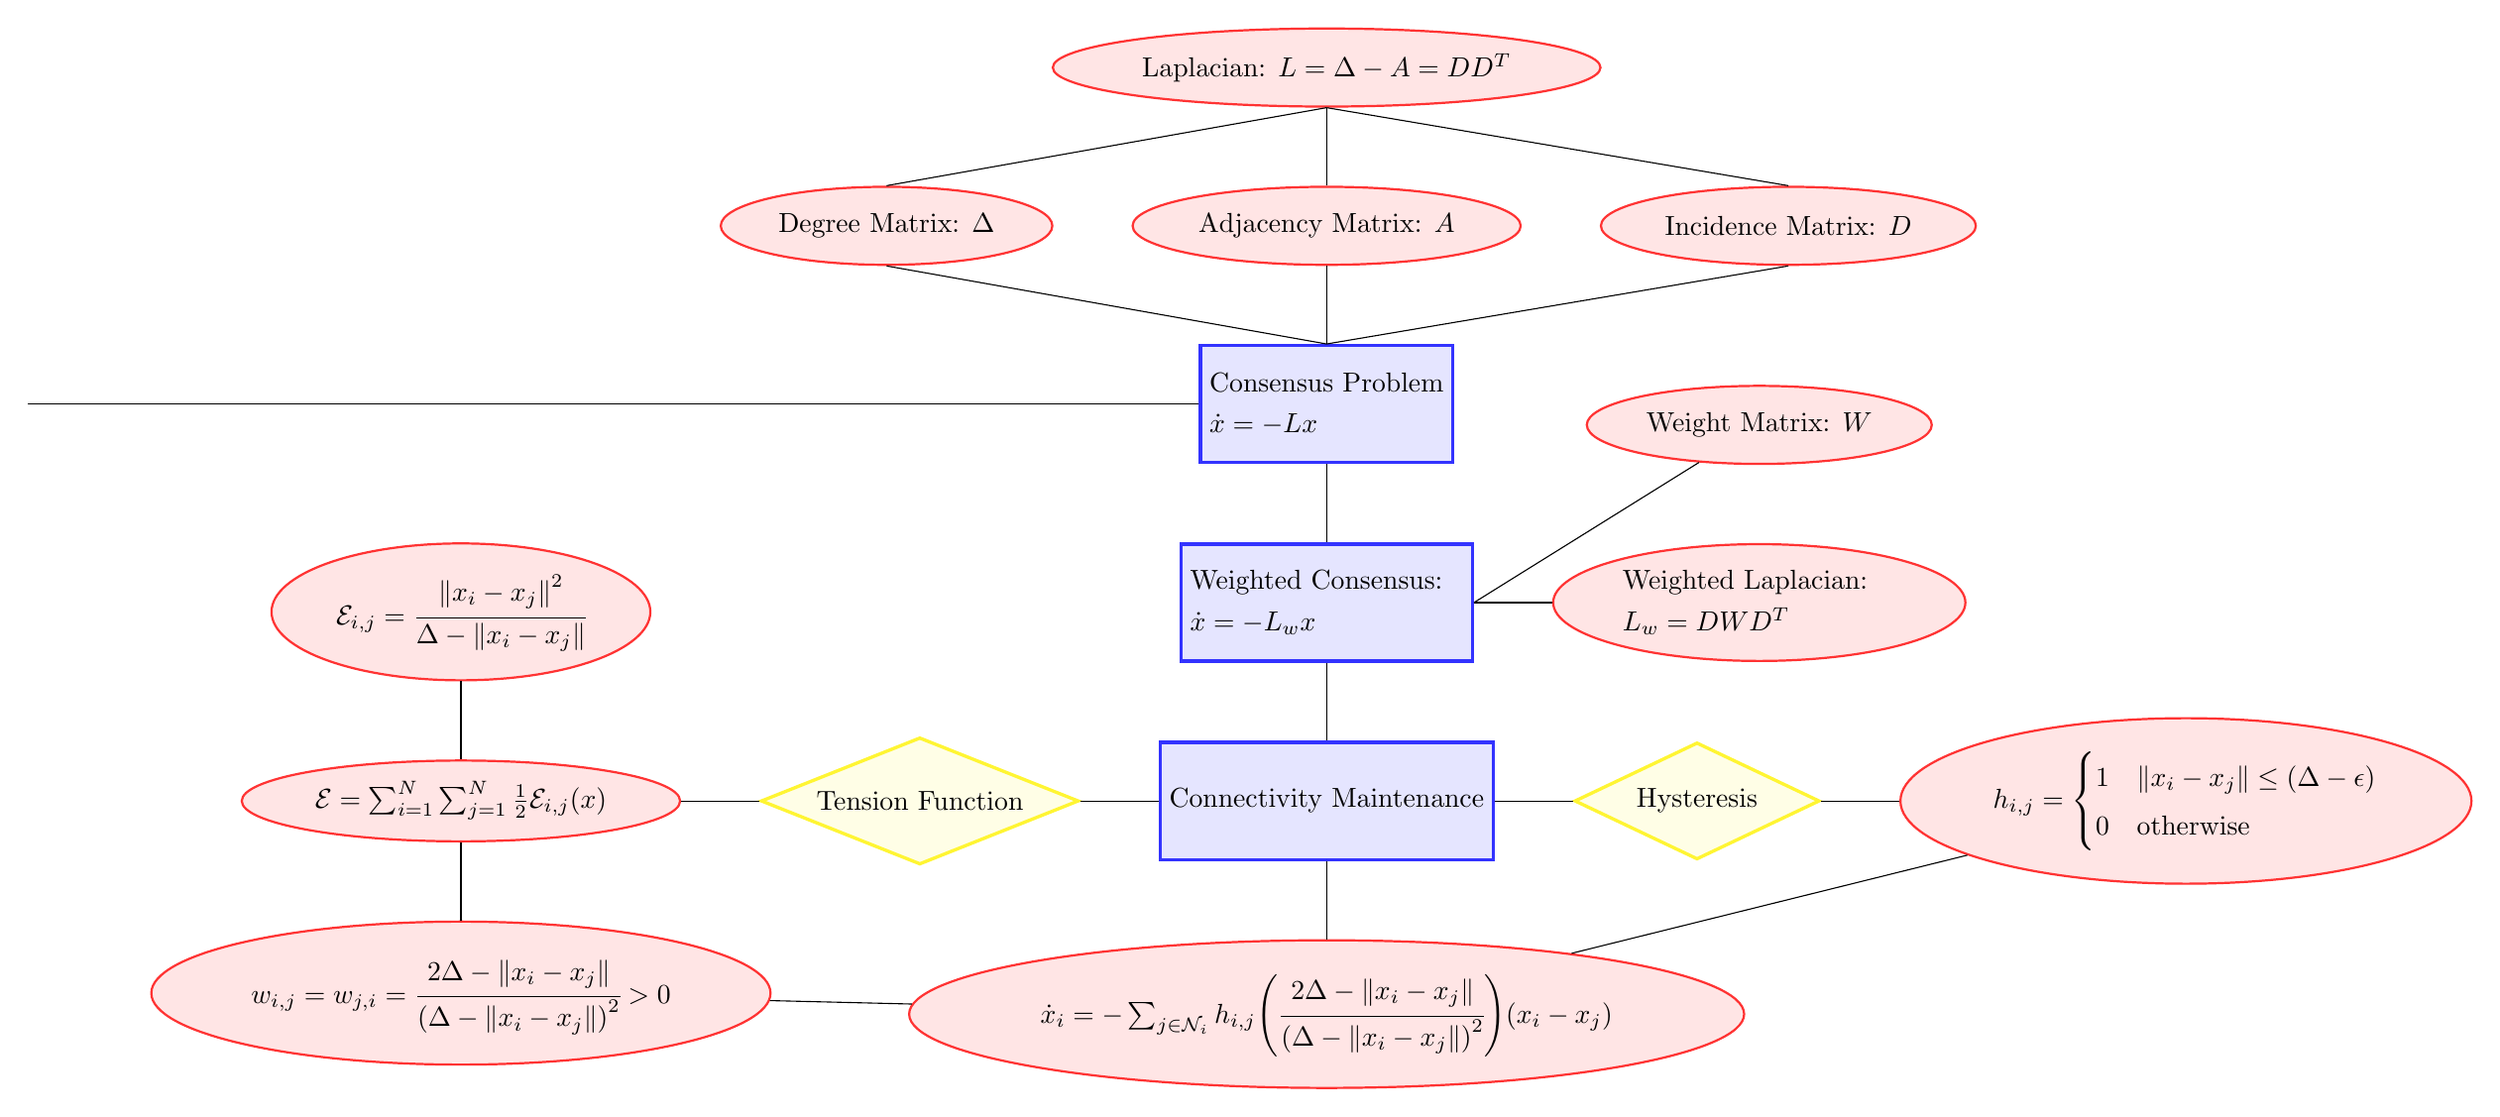
\begin{tikzpicture}[
		empty/.style={coordinate, draw=white!0, fill=white!0, thin, minimum size = 0.1mm},
		block/.style={rectangle, draw=blue!80, fill=blue!10, very thick, minimum size = 15mm},
        subblock/.style={diamond, draw=yellow!80, fill=yellow!10, very thick, minimum size = 15mm, aspect=2.5},
		extra/.style={ellipse, draw=red!80, fill=red!10, thick, minimum size = 10mm},
		auto,
		% roundnode/.style={circle, draw=green!60, fill=green!5, very thick, minimum size=7mm},
		% squarednode/.style={rectangle, draw=red!60, fill=red!5, very thick, minimum size=5mm},
		]
		%Main Nodes
		\node[empty]	(center)								{};
		
        % %Consensus
        \node[block, text width = 30mm]	(consensus)	[above=2cm of center]	{Consensus Problem $\dot{x}=-L x$};
        \node[extra]	(con_2)		[above=of consensus]	{Adjacency Matrix: $A$};
        \node[extra]	(con_1)		[left=of con_2]			{Degree Matrix: $\Delta$};
        \node[extra]	(con_3)		[right=of con_2]		{Incidence Matrix: $D$};
        \node[extra]	(con_4)		[above=of con_2]		{Laplacian: $L = \Delta - A = DD^T$};
        \draw[-]	(consensus.north) 	--	(con_1.south);
        \draw[-]	(consensus.north) 	--	(con_2.south);
        \draw[-]	(consensus.north) 	--	(con_3.south);
        \draw[-]	(con_1.north)		--	(con_4.south);
        \draw[-]	(con_2.north)		--	(con_4.south);
        \draw[-]	(con_3.north)		--	(con_4.south);

        % %Directed Consensus
        % \node[subblock]	(di_con)	[right=of consensus]	{Directed Consensus};
        % \draw[-]    (consensus.east) -- (di_con.west);
        % \node[extra]    (di_con_1)  [right=of di_con]    {Strongly vs Weakly Connected};
        % \draw[-]    (di_con.east) -- (di_con_1.west);
        % \node[extra]    (di_con_2)  [below=of di_con_1]    {Rooted Out-branching};
        % \draw[-]    (di_con.east) -- (di_con_2.west);

        %Weighted Consensus
        \node[block, text width = 35mm]	(w_con)	[below=of consensus]	{Weighted Consensus: $\dot{x} = -L_{w} x$};
        \draw[-]    (consensus.south) -- (w_con);
        \node[extra, text width = 35mm]    (w_con_2)  [right=of w_con]    {Weighted Laplacian: $L_{w} = D W D^{T}$};
        \draw[-]    (w_con.east) -- (w_con_2);
        \node[extra]    (w_con_1)  [above=of w_con_2]    {Weight Matrix: $W$};
        \draw[-]    (w_con.east) -- (w_con_1);
        % \node[extra]    (w_con_3)  [below=of w_con_2]    {Static \& Dynamic Weights};
        % \draw[-]    (w_con.east) -- (w_con_3.west);

        % %Time-Varying Consensus
        % \node[subblock]	(tv_con)	[left=of consensus]	{Time Varying Consensus};
        % \draw[-]    (consensus.west) -- (tv_con.east);
        % \node[extra]    (tv_con_1) [left=of tv_con] {Switched Networks};
        % \draw[-]    (tv_con.west) -- (tv_con_1.east);
        % \node[extra, text width = 40mm]    (tv_con_2) [below=of tv_con_1] {Universal vs Existential Stability};
        % \draw[-]    (tv_con.west) -- (tv_con_2.east);

        % %Lyapnov Stability
        % \node[block]	(lyap)		[left=3cm of center] 	{Lyapnov Stability};
        % \draw[-]    (lyap.west) -- (tv_con_2.east);
        % \draw[-]    (lyap.north) -- (consensus.south);

        % %Leader-Follower System
        % \node[block]	(lead_follow)		[right=3cm of center] 	{Leader-Follower Network};
        % \draw[-] (consensus.south) -- (lead_follow.north);

        %Connectivity Maintenance
        \node[block]	(cnct_maint)    [below=of w_con] 	{Connectivity Maintenance};
        \draw[-] (w_con.south) -- (cnct_maint.north);
        % Ten fun
        \node[subblock] (ten_fun) [left=of cnct_maint] {Tension Function};
        \draw[-] (cnct_maint) -- (ten_fun);
        \node[extra] (ten_fun_1) [left=of ten_fun] {$\mathcal{E} = \sum_{i=1}^{N} \sum_{j=1}^{N} \frac{1}{2} \mathcal{E}_{i,j}(x)$};
        \draw[-] (ten_fun) -- (ten_fun_1);
        \node[extra] (ten_fun_2) [above=of ten_fun_1] {$\mathcal{E}_{i,j} = \cfrac{\norm{x_i - x_j}^2}{\Delta - \norm{x_i - x_j}}$};
        \draw[-] (ten_fun_1) -- (ten_fun_2);
        \node[extra] (ten_fun_3) [below=of ten_fun_1] {$w_{i,j} = w_{j,i} =  \cfrac{2\Delta - \norm{x_i - x_j}}{\qty(\Delta - \norm{x_i - x_j})^2} > 0$};
        \draw[-] (ten_fun_1) -- (ten_fun_3);
        % Hysteresis
        \node[subblock] (hyst) [right=of cnct_maint] {Hysteresis};
        \draw[-] (cnct_maint) -- (hyst);
        \node[extra] (hyst_1) [right=of hyst] {$h_{i,j} = \begin{cases}
            1 &\norm{x_i - x_j} \leq (\Delta - \epsilon)\\
            0 &\text{otherwise}
        \end{cases}$};
        \draw[-] (hyst) -- (hyst_1);
        % Consensus eq
        \node[extra] (cnct_maint_1) [below=of cnct_maint] {$\dot{x}_i = - \sum_{j \in \mathcal{N}_i} h_{i,j} \qty(\cfrac{2\Delta - \norm{x_i - x_j}}{\qty(\Delta - \norm{x_i - x_j})^2}) (x_i - x_j)$};
        \draw[-] (cnct_maint) -- (cnct_maint_1);
        \draw[-] (ten_fun_3) -- (cnct_maint_1);
        \draw[-] (hyst_1) -- (cnct_maint_1);
		% %Applications
        % \node[subblock] (app) [below=2cm of center] {Applications};
        % % \draw[-] (lead_follow.south) -- (app.north);
        % % \draw[-] (lyap.south) -- (app.north);
		% \node[extra]	(app_2)		[below=of app]	    {Distributed Estimation};
		% \node[extra]	(app_1)		[left=of app_2]		{Flocking};
		% \node[extra]	(app_3)		[right=of app_2]	{Alignment};
		% \draw[-]	(app.south) -- (app_1.north);
		% \draw[-]	(app.south) -- (app_2.north);
		% \draw[-]	(app.south) -- (app_3.north);




        % Rigidity



        



        % Additional connections
        \node[empty] (p1) [left=150mm of consensus] {};
        \draw[-] (consensus) -- (p1);


	\end{tikzpicture}}
	\caption{Diagram of Course Topics (created w/ TikZ)}
	\label{fig:pblm1}
\end{figure}

% Problem 2 -------------------------------------------------
\newpage
\section{}

















\newpage
\appendix
\section{MATLAB Code:}\label{apx:matlab}
All code I write in this course can be found on my GitHub repository:\\
\href{https://github.com/jonaswagner2826/MECH6V29_MultiagentRoboticSystems}{https://github.com/jonaswagner2826/MECH6V29\_MultiagentRoboticSystems}

% \bibliographystyle{ieeetran}
% % \bibliography{refs.bib}
% \cite{*}

% \includepdf[pages=-]{MECH6V29_HW02.pdf}
% \includepdf[pages=-, nup = 2x2]{MECH6V29_HW02.pdf}


\end{document}
